%%%%%%%%%%%%%%%%%%%%%%%%%%%%%%%%%%%%%%%%%
% Structured General Purpose Assignment
% LaTeX Template
%
% This template has been downloaded from:
% http://www.latextemplates.com
%
% Original author:
%  Ted Pavlic (http://www.tedpavlic.com)
% Modified by:
%  Joe Del Rocco (https://joe.delrocco.org)
%%%%%%%%%%%%%%%%%%%%%%%%%%%%%%%%%%%%%%%%%

%----------------------------------------------------------------------------------------
%  PACKAGES AND CONFIGURATION
%----------------------------------------------------------------------------------------

\documentclass[fleqn]{article}
\usepackage{geometry}
\usepackage{fancyhdr} % For custom headers
\usepackage{lastpage} % To determine the last page for the footer
\usepackage{extramarks} % For headers and footers
\usepackage[most]{tcolorbox} % For problem answer sections
\usepackage{graphicx} % For inserting images
\usepackage{xcolor} % For link coloring
\usepackage[hidelinks]{hyperref} % For URL links (no box or color name)
\usepackage{bm}
\usepackage{amsmath}
\usepackage{amssymb}
\usepackage[english]{babel}
\usepackage[utf8x]{inputenc}
\usepackage{amsmath}
\usepackage{tikz}
\usetikzlibrary{arrows,automata}

% Margins
\geometry{
a4paper,
tmargin=1in,
bmargin=1in,
lmargin=1in,
rmargin=1in,
textwidth=6.5in,
textheight=9.0in,
headsep=0.25in
}

% Header and footer
\pagestyle{fancy}
\lhead{\myName} % Top left header
\chead{\myCourse: \myAssignment} % Top center header
\rhead{\firstxmark} % Top right header
\lfoot{\lastxmark} % Bottom left footer
\cfoot{} % Bottom center footer
\rfoot{Page\ \thepage\ of\ \pageref{LastPage}} % Bottom right footer
\renewcommand\headrulewidth{0.4pt} % Size of the header rule
\renewcommand\footrulewidth{0.4pt} % Size of the footer rule

% Other configurations
\setlength\parindent{0pt} % Removes all indentation from paragraphs
\setlength\parskip{1pt} % Ensures paragraphs are still recognizable as such
\setcounter{secnumdepth}{0} % Removes default section numbers
\setcounter{tocdepth}{3} % Sets depth of table of contents
\linespread{1.1}

% Template values
% \newcommand{\myLogo}{starfleet.jpg}
\newcommand{\myName}{Manish Yadav}
\newcommand{\myJobTitle}{3836-6483}
\newcommand{\myCompany}{Starfleet Academy}
\newcommand{\myLocation}{1701 Lincoln Blvd, San Francisco, CA}
\newcommand{\myURL}{www.starfleet.edu}
\newcommand{\myEmail}{m.yadav@ufl.edu}
\newcommand{\myCourse}{CNT5106C}
\newcommand{\mySection}{Fall 2020}
\newcommand{\myTeacher}{Dr. Ye Xia}
\newcommand{\myAssignment}{Homework 4}
\newcommand{\myDueDate}{Tue,\ Nov\ 3,\ 2020}
\newcommand{\norm}[1]{\left\lVert#1\right\rVert}


%----------------------------------------------------------------------------------------
%  DOCUMENT STRUCTURE (MACROS & ENVIRONMENTS)
%----------------------------------------------------------------------------------------

% Colored links macro
\newcommand{\hrefcol}[3] {\href{#1}{\textcolor{#3}{#2}}}

% Creates a counter to keep track of the number of problems
\newcounter{homeworkProblemCounter}

% Macro for custom title page signature header
\newsavebox{\myTitleSignature}
\sbox{\myTitleSignature}{%
\begin{tabular*}{\textwidth}{@{}l@{}@{\extracolsep{0.125in}}l@{}}%
\parbox[c][]{2.5in}{{\textbf{\myName} \par}
                    {\small \myJobTitle \par}
                    {\small \hrefcol{mailto:\myEmail}{\myEmail}{blue}} \par}
\end{tabular*}}

% Header and footer for when a page split occurs within a problem environment
\newcommand{\enterProblemHeader}[1]{%
\nobreak\extramarks{#1}{#1 continued on next page\ldots}\nobreak%
\nobreak\extramarks{#1 (continued)}{#1 continued on next page\ldots}\nobreak%
}

% Header and footer for when a page split occurs between problem environments
\newcommand{\exitProblemHeader}[1]{%
\nobreak\extramarks{#1 (continued)}{#1 continued on next page\ldots}\nobreak%
\nobreak\extramarks{#1}{}\nobreak%
}

\newcommand{\homeworkProblemName}{} % Argument = name of problem; default = "Problem #"
\newenvironment{homeworkProblem}[1][Problem \arabic{homeworkProblemCounter}]{%
\stepcounter{homeworkProblemCounter}% % Increase counter for number of problems
\renewcommand{\homeworkProblemName}{#1}% % Assign \homeworkProblemName the argument
\section{\homeworkProblemName}% % Make a section in the document with the custom problem count
\enterProblemHeader{\homeworkProblemName}% % Header and footer within environment
}{%
\exitProblemHeader{\homeworkProblemName}% % Header and footer after environment
}

\newcommand{\problemAnswer}[1]{ % Defines the problem answer command with the content as the only argument
\begin{tcolorbox}[breakable,enhanced,colback=gray!5!white,title=Answer]%
#1
\end{tcolorbox}%
% Alternative - Makes the box around the problem answer and puts the content inside
%\noindent\framebox[\columnwidth][c]{\begin{minipage}{0.98\columnwidth}#1\end{minipage}}
}

\newcommand{\homeworkSectionName}{}
\newenvironment{homeworkSection}[1]{% % For sections w/in problems; Argument = name of section (no default)
\renewcommand{\homeworkSectionName}{#1}% % Assign \homeworkSectionName the argument
\subsection{\homeworkSectionName}% % Make a subsection with the name of the subsection
\enterProblemHeader{\homeworkProblemName\ [\homeworkSectionName]}% % Header and footer within environment
}{%
\enterProblemHeader{\homeworkProblemName}% % Header and footer after environment
}

%----------------------------------------------------------------------------------------
%   TITLE PAGE
%----------------------------------------------------------------------------------------
\begin{document}

% Blank out the traditional title page
\title{\vspace{-1in}} % no title name
\author{} % no author name
\date{} % no date listed
\maketitle % makes this a title page

% Use custom title macro instead
\usebox{\myTitleSignature}
\vspace{1in} % spacing below title header

% Assignment title
{\centering \huge \myAssignment \par}
{\centering \noindent\rule{4in}{0.1pt} \par}
\vspace{0.05in}
{\centering \myCourse~: \mySection~: \myTeacher \par}
{\centering Due \myDueDate \par}
%{\centering Prepared w/ \LaTeX \par}
\vspace{1in}

% Table of Contents
\tableofcontents
\newpage

%----------------------------------------------------------------------------------------
%	PROBLEM 1
%----------------------------------------------------------------------------------------

%\begin{homeworkProblem}[Exercise \#\arabic{homeworkProblemCounter}] % Use for custom section title
\begin{homeworkProblem}
\begin{homeworkSection}{P31}
Suppose that the five measured \texttt{SampleRTT} values (see Section 3.5.3 ) are 106 ms, 120 ms, 140 ms, 90 ms, and 115 ms. Compute the \texttt{EstimatedRTT} after each of these \texttt{SampleRTT} values is obtained, using a value of $\alpha=0.125$ and assuming that the value of \texttt{EstimatedRTT} was 100 ms just before the first of these five samples were obtained. Compute also the \texttt{DevRTT} after each sample is obtained, assuming a value of $\beta = 0.25$ and assuming the value of \texttt{DevRTT} was 5 ms just before the first of these five samples was obtained. Last, compute the TCP \texttt{TimeoutInterval} after each of these samples is obtained \\
\problemAnswer{
    \begin{itemize}
        \item For RTT = 106ms
        \begin{align*}
                \texttt{EstimatedRTT} &= \alpha * \texttt{SampleRTT} + (1 - \alpha) * \texttt{EstimatedRTT} \\
                &= 0.125 * 106 + (1 - 0.125) * 100 \\
                &= 0.125* 106 + 0.875 * 100 \\
                &= 100.75ms
        \end{align*}
        \begin{align*}
                \texttt{DevRTT} &= \beta * |{\texttt{SampleRTT} - \texttt{EstimatedRTT}}| + (1 - \beta) * \texttt{DevRTT} \\
                &= 0.25 * |106-100.75| + (1-0.25) *5 \\
                &= 0.125* 106 + 0.875 * 100 \\
                &= 5.06ms
        \end{align*}
        \begin{align*}
                \texttt{TCPTimeoutInterval} &= \texttt{EstimatedRTT} + 4 * \texttt{DevRTT} \\
                &= 100.75 + 4 *5.0625 \\
                &= 121ms
        \end{align*}
        \item For RTT = 120ms
        \begin{align*}
                \texttt{EstimatedRTT} &= \alpha * \texttt{SampleRTT} + (1 - \alpha) * \texttt{EstimatedRTT} \\
                &= 0.125 * 120 + (1-0.125) * 100.75 \\
                &= 103.15ms
        \end{align*}
        \begin{align*}
                \texttt{DevRTT} &= \beta * |{\texttt{SampleRTT} - \texttt{EstimatedRTT}}| + (1 - \beta) * \texttt{DevRTT} \\
                &= 0.25 * |120-103.15625| + (1-0.25) *5.0625 \\
                &= 8ms
        \end{align*}
        \begin{align*}
                \texttt{TCPTimeoutInterval} &= \texttt{EstimatedRTT} + 4 * \texttt{DevRTT} \\
                &= 103.15 + 4 *8  \\
                &= 135.15ms
        \end{align*}
        \item For RTT = 140ms
        \begin{align*}
                \texttt{EstimatedRTT} &= \alpha * \texttt{SampleRTT} + (1 - \alpha) * \texttt{EstimatedRTT} \\
                &= 0.125 * 140 + (1-0.125) * 103.15 \\
                &= 107.75ms
        \end{align*}
        \begin{align*}
                \texttt{DevRTT} &= \beta * |{\texttt{SampleRTT} - \texttt{EstimatedRTT}}| + (1 - \beta) * \texttt{DevRTT} \\
                &= 0.25 * |140-107.75| + (1-0.25) *8\\
                &= 14.06ms
        \end{align*}
        \begin{align*}
                \texttt{TCPTimeoutInterval} &= \texttt{EstimatedRTT} + 4 * \texttt{DevRTT} \\
                &= 107.75 + 4 *14.06 \\
                &= 164ms
        \end{align*}
        \item For RTT = 90ms
        \begin{align*}
                \texttt{EstimatedRTT} &= \alpha * \texttt{SampleRTT} + (1 - \alpha) * \texttt{EstimatedRTT} \\
                &= 0.125 * 90 + (1-0.125) * 107.75 \\
                &= 105.53ms
        \end{align*}
        \begin{align*}
                \texttt{DevRTT} &= \beta * |{\texttt{SampleRTT} - \texttt{EstimatedRTT}}| + (1 - \beta) * \texttt{DevRTT} \\
                &=  0.25 * |90-105.53| + (1-0.25) *14.06\\
                &= 14.42ms
        \end{align*}
        \begin{align*}
                \texttt{TCPTimeoutInterval} &= \texttt{EstimatedRTT} + 4 * \texttt{DevRTT} \\
                &= 105.53 + 4 *14.42\\
                &= 163.21ms
        \end{align*}
        \item For RTT = 115ms
        \begin{align*}
                \texttt{EstimatedRTT} &= \alpha * \texttt{SampleRTT} + (1 - \alpha) * \texttt{EstimatedRTT} \\
                &= 0.125 * 115 + (1-0.125) * 105.53 \\
                &= 106.715ms
        \end{align*}
        \begin{align*}
                \texttt{DevRTT} &= \beta * |{\texttt{SampleRTT} - \texttt{EstimatedRTT}}| + (1 - \beta) * \texttt{DevRTT} \\
                &=  0.25 * |115-106.715| + (1-0.25) *14.42 \\
                &= 12.885ms
        \end{align*}
        \begin{align*}
                \texttt{TCPTimeoutInterval} &= \texttt{EstimatedRTT} + 4 * \texttt{DevRTT} \\
                &= 106.715 + 4 *12.885 \\
                &= 158.255ms
        \end{align*}
    \end{itemize}
}
\end{homeworkSection}
\end{homeworkProblem}
%----------------------------------------------------------------------------------------
\pagebreak

\begin{homeworkProblem}
Consider Figure 3.58 . Assuming TCP Reno is the protocol experiencing the behavior shown above, answer the following questions. In all cases, you should provide a short discussion justifying your answer.
\begin{homeworkSection}{P40 a}
Identify the intervals of time when TCP slow start is operating. \\
\problemAnswer{
    [1,6] and [23,16]
}
\end{homeworkSection}

\begin{homeworkSection}{P40 b}
Identify the intervals of time when TCP congestion avoidance is operating. \\
\problemAnswer{
    [6, 16] and [7, 22]
}
\end{homeworkSection}

\begin{homeworkSection}{P40 c}
After the 16th transmission round, is segment loss detected by a triple duplicate ACK or by a timeout? \\
\problemAnswer{
    It would be triple duplicate ACK. In case of timeout, congestion size would have been reduced.
}
\end{homeworkSection}

\begin{homeworkSection}{P40 d}
After the 22nd transmission round, is segment loss detected by a triple duplicate ACK or by a timeout? \\
\problemAnswer{
    It is detected due to timeout as the congestion window size is 1
}
\end{homeworkSection}

\begin{homeworkSection}{P40 e}
What is the initial value of \texttt{ssthresh} at the first transmission round? \\
\problemAnswer{
    32 (At this size, slow start stops and congestion avoidance begins)
}
\end{homeworkSection}

\begin{homeworkSection}{P40 f}
What is the value of \texttt{ssthresh} at the 18th transmission round? \\
\problemAnswer{
    $\frac{42}{2} = 21$
}
\end{homeworkSection}

\begin{homeworkSection}{P40 g}
What is the value of \texttt{ssthresh} at the 24th transmission round? \\
\problemAnswer{
    $\frac{29}{2} = 14$
}
\end{homeworkSection}

\begin{homeworkSection}{P40 h}
During what transmission round is the 70th segment sent? \\
\problemAnswer{
    \begin{itemize}
        \item Transmission round 1: $pkt_1$
        \item Transmission round 2: $pkt_{2-3}$
        \item Transmission round 3: $pkt_{4-7}$
        \item Transmission round 4: $pkt_{8-16}$
        \item Transmission round 5: $pkt_{17-32}$
        \item Transmission round 6: $pkt_{33-63}$
        \item Transmission round 7: $pkt_{64-96}$
    \end{itemize}
    Therefore $pkt_70$ is sent in round 7
}
\end{homeworkSection}

\begin{homeworkSection}{P40 i}
Assuming a packet loss is detected after the 26th round by the receipt of a triple duplicate ACK, what will be the values of the congestion window size and of \texttt{ssthresh} ? \\
\problemAnswer{
    %% Doubt
    Congestion window size = $\frac{8}{2} + 3 = 7$ \\
    \texttt{ssthresh} = $\frac{8}{2} = 4$
}
\end{homeworkSection}

\begin{homeworkSection}{P40 j}
Suppose TCP Tahoe is used (instead of TCP Reno), and assume that triple duplicate ACKs are received at the 16th round. What are the ssthresh and the congestion window size at the 19th round? \\
\problemAnswer{
    \texttt{ssthresh} = 21\\
    Congestion Window Size = 1
}
\end{homeworkSection}

\begin{homeworkSection}{P40 k}
Again suppose TCP Tahoe is used, and there is a timeout event at 22nd round. How many packets have been sent out from 17th round till 22nd round, inclusive? \\
\problemAnswer{
    \begin{itemize}
        \item Round 17: 1 packet
        \item Round 18: 2 packets
        \item Round 19: 4 packets
        \item Round 20: 8 packets
        \item Round 21: 16 packets
        \item Round 22: 21 packets
    \end{itemize}
}
\end{homeworkSection}
\end{homeworkProblem}
%----------------------------------------------------------------------------------------
\pagebreak

\begin{homeworkProblem}
\begin{homeworkSection}{P41}
Refer to Figure 3.55 , which illustrates the convergence of TCP’s AIMD algorithm. Suppose that instead of a multiplicative decrease, TCP decreased the window size by a constant amount.
Would the resulting AIAD algorithm converge to an equal share algorithm? Justify your answer using a diagram similar to Figure 3.55. \\

\problemAnswer{
    \begin{center}
        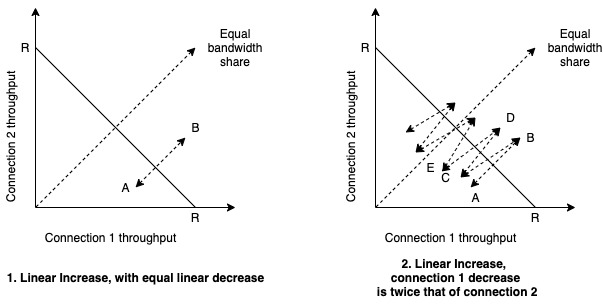
\includegraphics[width=\columnwidth]{47.jpg}
    \end{center}
    In fig 1, the ratio of linear decrease on loss of connection 1 and connection 2 is proportional to ratio of linear increase of connection 1 and connection. Hence there is no fluctuation of throughput and it stays on line AB. \\
    
    In fig 2, linear decrease on loss between connection 1 and 2 is proportional to 2:1 i.e. whenever there is a loss, window size on connection 1 reduces by 2 times the window size of connection 2. Subsequently, the repeats and after few increase and decrease in losses, connection 1 throughput goes to 0 and full bandwidth is allocated for connection 2.
}
\end{homeworkSection}
\end{homeworkProblem}
%----------------------------------------------------------------------------------------
\pagebreak

\begin{homeworkProblem}
Consider sending a large file from a host to another over a TCP connection that has no loss. \\
\begin{homeworkSection}{P44 a}
Suppose TCP uses AIMD for its congestion control without slow start. Assuming cwnd increases by 1 MSS every time a batch of ACKs is received and assuming approximately constant round-trip times, how long does it take for cwnd increase from 6 MSS to 12 MSS (assuming no loss events)? \\
\problemAnswer{
After 1 RTT, Congestion Window is set to 6 MMS, each ACKs increases it by 1; therefore by 2 RTT it is 7 MSS, 3 RTTs to 8 MSS and so on so forth.
After 7 RTTs, it is increased to 12 MSS.
}
\end{homeworkSection}

\begin{homeworkSection}{P44 b}
What is the average throughout (in terms of MSS and RTT) for this connection up through time=6 RTT? \\
\problemAnswer{
    \begin{itemize}
        \item RTT 1: 5 MSS sent
        \item RTT 2: 6 MSS sent
        \item RTT 3: 7 MSS sent
        \item RTT 4: 8 MSS sent
        \item RTT 5: 9 MSS sent
        \item RTT 6: 10 MSS sent
    \end{itemize}
    
    Total MSS Sent = $5 + 6 + 7 + 8 + 9 + 10 = 45 MSS$. Therefore average throughput = $\frac{45}{6} = 7.5 MSS/RTT$
}
\end{homeworkSection}
\end{homeworkProblem}
%----------------------------------------------------------------------------------------
\pagebreak

\begin{homeworkProblem}
Recall the macroscopic description of TCP throughput. In the period of time from when the connection’s rate varies from W/(2 · RTT) to W/RTT, only one packet is lost (at the very end of the period).
\begin{homeworkSection}{P45 a}
Show that the loss rate (fraction of packets lost) is equal to L=loss rate= $\frac{1}{\frac{3}{8}W^2 + \frac{3}{4}W}$ \\
\problemAnswer{
    Loss Ratio = Number of packets lost over number of packets sent\\
    
    The packets send in each round is given using the equation:
    
    \begin{align*}
        &= \frac{W}{2} + (\frac{W}{2} + 1) + ... + W) \\
        &= \sum_{n = 0}^{W/2} (\frac{W}{2} + n) \\
        &= (\frac{W}{2} + 1) \frac{W}{2} + \frac{\frac{W}{2} (W/2 + 1)}{2} \\
        &= \frac{W^2}{4} + \frac{W}{2} + \frac{W^2}{8} + \frac{W}{4}\\
        &= \frac{3}{8}W^2 + \frac{3}{4}W
    \end{align*}
    \\
    
    Therefore loss rate = $\frac{1}{\frac{3}{8}W^2 + \frac{3}{4}W}$
}
\end{homeworkSection}

\begin{homeworkSection}{P45 b}
Use the result above to show that if a connection has loss rate L, then its average rate is approximately given by ≈ $\frac{1.22 \cdot MSS}{RTT \cdot \sqrt{L}}$ \\
\problemAnswer{
    For sufficiently large value of W, $\frac{3W^2}{8} >> \frac{3W}{4}$, therefore loss rate is dependent on $\frac{8W^2}{3}$ i.e. $W = \sqrt{\frac{8}{3 L}}$
    
    Therefore average throughput = $\frac{3}{4} \sqrt{\frac{8}{3L}}\frac{MSS}{RTT} = \frac{1.22 MSS}{RTT\sqrt{L}}$
}
\end{homeworkSection}
\end{homeworkProblem}
%----------------------------------------------------------------------------------------
\pagebreak

\begin{homeworkProblem}
\begin{homeworkSection}{P47}
Consider the scenario described in the previous problem. Suppose that the 10Mbps link can buffer a finite number of segments. Argue that in order for the link to always be busy sending data, we would like to choose a buffer size that is at least the product of the link speed C and the two-way propagation delay between the sender and the receiver. \\
\problemAnswer{
    Assuming W to be max window size and S to be buffer size. 
    Assuming TCP to be operating in round by round fashion. One round = 1 RTT. Packet loss will occur when the window size reaches W, in this scenario, sender would reduce the congestion window size by $\frac{1}{2}$ and wait for the ACKs of remaining $\frac{W}{2}$ packets before it begin sending data again.
    By sending data every W/(2*C) period, we keep the link busy. This is when where the sender waits for the ACKs from W/2 packets. Therefore S/C $\geq $ W/2.\\
    
    Upon reaching window size of W/2 and emptying the buffer, we need to be sure that link is busy sending data as well. There we need to ensure that $\frac{\frac{W}{2}}{2T_p} \geq C$ i.e. $\frac{W}{2} \geq C*2T_p$ i.e. $S \geq C*2T_p$ where $T_p$ is propagation delay between sender and receiver.
}
\end{homeworkSection}
\end{homeworkProblem}
%----------------------------------------------------------------------------------------
\pagebreak

\begin{homeworkProblem}
\textbf{Wireshark Lab: TCP}
\begin{homeworkSection}{1}
What is the IP address and TCP port number used by the client computer (source) that is transferring the file to gaia.cs.umass.edu? \\
\problemAnswer{
    IP address: 192.168.1.102 \\
    TCP port number: 1161
}
\end{homeworkSection}

\begin{homeworkSection}{2}
What is the IP address of gaia.cs.umass.edu? On what port number is it sending and receiving TCP segments for this connection?
\problemAnswer{
    IP address: 128.119.245.12\\
    Port: 80
}
\end{homeworkSection}

\begin{homeworkSection}{3}
What is the IP address of gaia.cs.umass.edu? On what port number is it sending and receiving TCP segments for this connection?
\problemAnswer{
    IP address: 10.76.65.181 \\
    Port: 80
}
\end{homeworkSection}

\begin{homeworkSection}{4}
What is the sequence number of the TCP SYN segment that is used to initiate the TCP connection between the client computer and gaia.cs.umass.edu?  What is it in the segment that identifies the segment as a SYN segment? \\
\problemAnswer{
    TCP SYN sequence number is 0. \\ SYN Flag in that segment is set to 1.
}
\end{homeworkSection}

\begin{homeworkSection}{5}
What is the sequence number of the SYNACK segment sent by gaia.cs.umass.edu to the client computer in reply to the SYN?  What is the value of the Acknowledgement field in the SYNACK segment?  How did gaia.cs.umass.edu determine that value? What is it in the segment that identifies the segment as a SYNACK segment? \\
\problemAnswer{
    SYNACK segment number is 0. \\
    Acknowledgement filed in the SYNACK segment is 1. \\
    The server adds 1 to the intial sequence number of SYN segment from the client computer. \\
    Both SYN flag and Acknowledgement in the segment are set to 1
}
\end{homeworkSection}

\begin{homeworkSection}{6}
What is the sequence number of the TCP segment containing the HTTP POST command?  Note that in order to find the POST command, you’ll need to dig into the packet content field at the bottom of the Wireshark window, looking for a segment with a “POST” within its DATA field. \\
\problemAnswer{
    TCP segment 6 contains the POST request. Sequence number is 1
}
\end{homeworkSection}

\begin{homeworkSection}{7}
Consider the TCP segment containing the HTTP POST as the first segment in the TCP connection. What are the sequence numbers of the first six segments in the TCP connection (including the segment containing the HTTP POST)?  At what time was each segment sent?  When was the ACK for each segment received?  Given the difference between when each TCP segment was sent, and when its acknowledgement was received, what is the RTT value for each of the six segments?  What is the EstimatedRTT value (see Section 3.5.3, page 242in text) after the receipt of each ACK?  Assume that the value of the EstimatedRTT is equal to the measured RTT for the first segment, and then is computed using the EstimatedRTT equation on page 242 for all subsequent segments \\
\problemAnswer{
    \begin{center}
        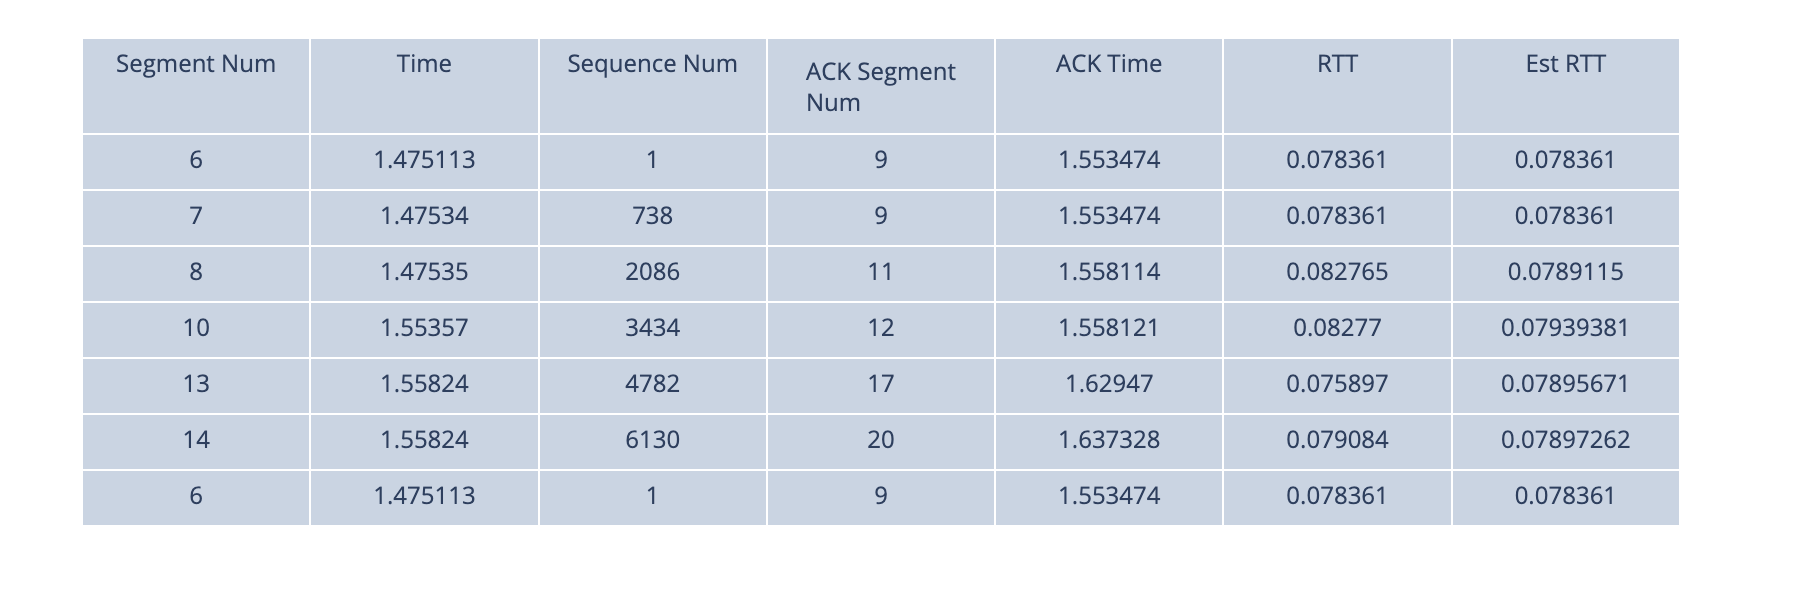
\includegraphics[width=\columnwidth]{TCP.png}
    \end{center}
}
\end{homeworkSection}

\begin{homeworkSection}{8}
What is the length of each of the first six TCP segments? \\
\problemAnswer{
    Segment Num 6: Sequence Num: 1, Length: 737\\
    Segment Num 7: Sequence Num: 738, Length: 1348\\
    Segment Num 8: Sequence Num: 2086, Length: 1348\\
    Segment Num 10: Sequence Num: 3434, Length: 1348\\
    Segment Num 13: Sequence Num: 4782, Length: 1348\\
    Segment Num 14: Sequence Num: 6130, Length: 1348\\
}
\end{homeworkSection}

\begin{homeworkSection}{9}
What is the minimum amount of available buffer space advertised at the received for the entire trace?  Does the lack of receiver buffer space ever throttle the sender? \\
\problemAnswer{
    Window Size = 28960.
    \begin{center}
        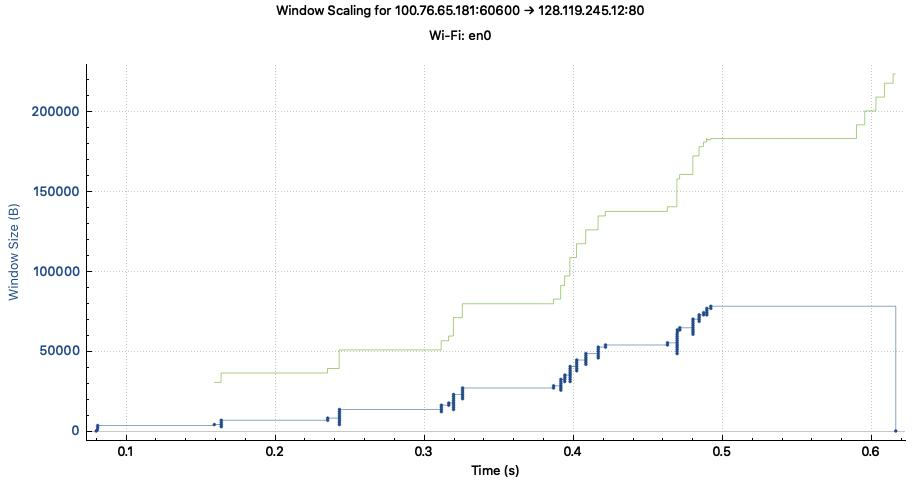
\includegraphics[width=\columnwidth]{9.jpeg}
    \end{center}
    As seen from figure there was no throttling
}
\end{homeworkSection}

\begin{homeworkSection}{10}
Are there any retransmitted segments in the trace file? What did you check for (in the trace) in order to answer this question? \\
\problemAnswer{
    There isn't seem to be any retransmitted segment. Retransmitted packet are highlighted using black color and there's none.
}
\end{homeworkSection}

\begin{homeworkSection}{11}
How much data does the receiver typically acknowledge in an ACK?  Can you identify cases where the receiver is ACKing every other received segment (see Table 3.2 on page 250 in the text). \\
\problemAnswer{
     The difference between the acknowledged sequence numbers of two consecutive ACKs indicates the data received by the server between these two ACKs. The receiver typically acknowledges 1400 - 2000 bytes. This almost triples is almost constant in the end as they are received in ordered fashion and hence ACKs every other segment.
}
\end{homeworkSection}

\begin{homeworkSection}{12}
What is the throughput (bytes transferred per unit time) for the TCP connection?  Explain how you calculated this value. \\
\problemAnswer{
    % Time taken to upload file = 2.01 (Last segment) - 1.39 (First segment) = 0.62s
    % Size of file = 152,138
    % Throughput = 152,138 / 0.6 = 253563.33 bytes/sec
    Throughput = 48k bytes/sec (As per file statistics)
}
\end{homeworkSection}

\begin{homeworkSection}{13}
Use the Time-Sequence-Graph(Stevens) plotting tool to view the sequence number versus time plot of segments being sent from the client to the gaia.cs.umass.edu server.  Can you identify where TCP’s slowstart phase begins and ends, and where congestion avoidance takes over?  Comment on ways in which the measured data differs from the idealized behavior of TCP that we’ve studied in the text. \\
\problemAnswer{
    We could slow start happening at 0-0.15s and then the sender transmits in the batches of 6. Now in this case we do not observe any linear increase in batch size. This is different from the one in text as it does not AIMD strategy as window size does not increase even when there is no congestion.
}
\end{homeworkSection}

\begin{homeworkSection}{14}
Answer each of two questions above for the trace that you have gathered when you transferred a file from your computer to gaia.cs.umass.edu\\ 
\problemAnswer{
    \begin{center}
        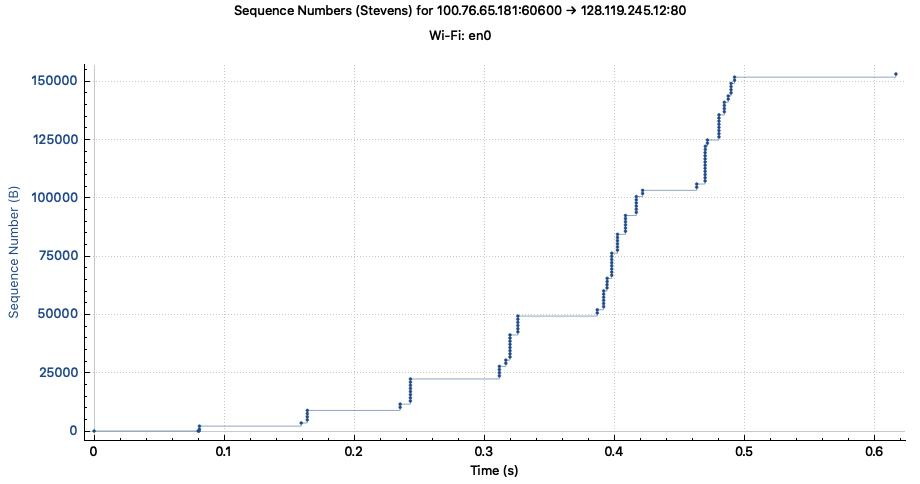
\includegraphics[width=\columnwidth]{steven.jpeg}
    \end{center}
    From the above stevens graph it is clear that congestion starts at 0ms but doesn't seem to end as file upload finishes even before congestion could happen or window slow start phase could. This behaviour is due higher bandwidth of my machine. Hence no comparison could be made with the one in text due to incomplete slow start behaviour.
}
\end{homeworkSection}
\end{homeworkProblem}
%----------------------------------------------------------------------------------------
\pagebreak
\bibliographystyle{plain}
\bibliography{references} % see references.bib for bibliography management
\end{document}
%----------------------------------------------------------------------------------------
%	DONE
%----------------------------------------------------------------------------------------
